\subsection{Dead Node Elimination}\label{sec:dne}

\begin{figure*}
	\subfloat[Code\label{fig:dcne-code}]{
		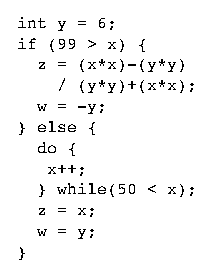
\includegraphics[scale=0.84]{code}
	}
	\hfill
	\subfloat[RVSDG\label{fig:dcne1}]{
		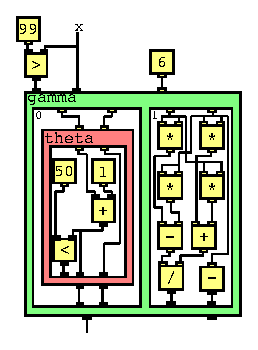
\includegraphics[scale=0.84]{dcne1}
	}
	\hfill
	\subfloat[After CNE\label{fig:dcne2}]{
		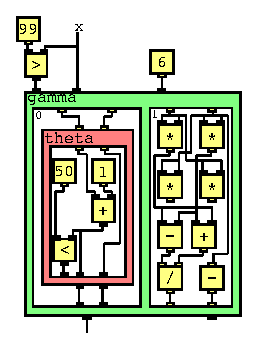
\includegraphics[scale=0.84]{dcne2}
	}
	\hfill
	\subfloat[After DNE mark\label{fig:dcne3}]{
		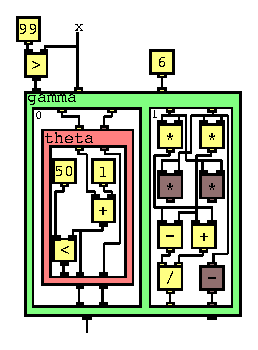
\includegraphics[scale=0.84]{dcne3}
	}
	\caption{Dead and Common Node Elimination}
	\label{fig:dcne}
\end{figure*}

Dead Node Elimination (DNE) is a combination of dead and unreachable code elimination, and removes
all nodes that do not contribute to the result of a computation. Dead nodes are generated by
unreachable and dead code from the input program, as well as by other
optimizations such as Common Node Elimination.
An operation is considered dead code when its results are either not used or only by
other dead operations. Thus, an output of a node is dead, if it has no users or all its users are
dead. We consider a node to be dead, if all its outputs are
dead. It follows that a node's inputs are dead, if the node itself is dead. We call all entities
that are not dead alive.

The implementation of DNE consists of two phases: mark and sweep. The mark phase identifies all
outputs and arguments that are alive, while the sweep phase removes all dead entities. The mark
phase traverses RVSDG edges according to the rules in Algorithm \ref{alg:dne}. If a structural
node is dead, the mark phase skips the traversal of its subregions as well as all of the contained
computations, as it never reaches the node in the first place. The mark phase is invoked for all
result origins of the \omegaregion.

The sweep phase performs a simple
bottom-up traversal of an RVSDG, recursively processing subregions of structural nodes as long as
these nodes are alive. A dead structural node is removed with all its contained computations.
The RVSDG's uniform representation of all computations as nodes permits DNE to not only remove
simple computations, but also compound computations such as conditionals, loops, or even entire
functions. Moreover, its nested structure avoids the processing of entire branches of the region
tree if they are dead.

\begin{informalg}{Dead Node Elimination}{alg:dne}
\begin{enumerate}
	\vspace*{-0.7\baselineskip}

	\item \bpoint{Mark}: Mark output or argument as alive and continue as follows:
		\begin{itemize}
			\item \bpoint{\omegaregion argument}: Stop marking.

			\item \bpoint{\phinode output}: Mark the result origin of the corresponding recursion
				variable.

			\item \bpoint{\phiregion argument}: Mark the input origin if the argument belongs to a
				context variable. Otherwise, mark the output of the corresponding recursion variable.

			\item \bpoint{\lambdanode output}: Mark all result origins of the \lambdaregion.

			\item \bpoint{\lambdaregion argument}: Mark the input origin if the argument is a dependency.

			\item \bpoint{\thetanode output}: Mark the \thetanode's predicate origin as well as the
				result and input origin of the corresponding loop variable.

			\item \bpoint{\thetaregion argument}: Mark the input origin and output of the corresponding
				loop variable.

			\item \bpoint{\gammanode output}: Mark the \gammanode's predicate origin as well as the
				origins of all results of the corresponding exit variable.

			\item \bpoint{\gammaregion argument}: Mark the input origin of the corresponding entry
				variable.

			\item \bpoint{Simple node output}: Mark the origin of all inputs.
		\end{itemize}

	\item \bpoint{Sweep}: Process all nodes in reverse topological order and remove them if they are
		dead. Otherwise, process them as follows:
		\begin{itemize}
			\item \bpoint{\omeganode}: Recursively process the \omegaregion. Remove all dead arguments.

			\item \bpoint{\gammanode}: For all exit variables $(R,o) \in EX$ where $o$ is dead, remove
				$o$ and all $r \in R$. Recursively process the \gammaregions. For all entry variables
				$(i,A) \in EV$ where all $a \in A$ are dead, remove all $a \in A$ and $i$.

			\item \bpoint{\thetanode}: For all loop variables $(i,a,r,o) \in LV$ where $a$ and $o$ are
				dead, remove $o$ and $r$. Recursively process the \thetaregion. Remove $i$ and $a$. 

			\item \bpoint{\lambdanode}: Recursively process the \lambdaregion. For all context variables
				$(i,a) \in CV$ where $a$ is dead, remove $a$ and $i$.

			\item \bpoint{\phinode}: For all recursion variables $(r, a, o) \in RV$ where $a$ and $o$ are
				dead, remove $o$ and $r$. Recursively process the \phiregion. Remove $a$. For all context
				variables $(i,a) \in CV$ where $a$ is dead, remove $a$ and $i$.
		\end{itemize}

	\vspace*{-\baselineskip}
\end{enumerate}
\end{informalg}

Figure~\ref{fig:dcne3} shows the RVSDG from Figure~\ref{fig:dcne2} after the mark phase.
Grey colored entities are dead. The mark phase traverses
the graph's edges, marking the \gammanode's leftmost output alive. This renders the
corresponding result origins of the \gammaregions alive, then the leftmost output of the
\thetanode, and so forth. After the mark phase annotated all outputs and arguments as alive, the
sweep phase removes all dead entities.

